\chapter{上位机软件研发与使用}
\label{app:pc-host}

上位机为 FPGA 图像矫正系统提供视频对照、运行时控制、Gamma 遥测、
IMU 姿态显示和图卡评估入口。本附录依据 \path{../PC/} 中的 Python 工程，
介绍软件结构、关键实现与联调方法。
软件以 Python 3.10 及以上版本、PySide6/Qt 为界面基础，
通过 OpenCV、NumPy 和 pyserial 完成图像分析、模型变换及串口通信。
现有版本为 0.1.0，使用的模型、协议和参考资料保存在 \path{Device/} 中。

\section{功能范围与设备连接}
\subsection{两路视频与两条串口}
系统由原始相机、PC 副屏、FPGA、HDMI 采集卡及 STM32 组成。
原始相机通过 USB 接入 PC，其实时图像可经副屏 HDMI 送入 FPGA；
FPGA HDMI 输出通过独立 USB 采集卡回到 PC，与原始预览并排显示。
PC 与 FPGA 的 CP210x 串口用于控制和统计，
PC 与 STM32 的 USB CDC 用于接收姿态；图像不经过这两条串口传输。

\begin{table}[htbp]\centering\small
\caption{上位机设备接口与数据用途}\label{tab:app-host-devices}
\begin{tabularx}{\textwidth}{>{\raggedright\arraybackslash}p{3.0cm}>{\raggedright\arraybackslash}p{3.0cm}Y}
\toprule
设备 & 识别参考 & 数据与连接要求 \\
\midrule
AR0234 USB 相机 & VID:PID \texttt{1bcf:2cd1} & 原始视频，目标采集请求 $1920\times1080$、60 fps \\
UGREEN 25854 & \texttt{2b89:5854} & 采集 FPGA HDMI 输出，独立于原相机视频节点 \\
FPGA CP210x & \texttt{10c4:ea60} & 115200/8-N-1，无流控；功能掩码、状态和 Gamma 统计 \\
STM32 Virtual COM & \texttt{0483:5740} & 115200/8-N-1 线路设置；十字节姿态协议 \\
PC 独立副屏 & 显示器名称与实际信号模式 & 扩展桌面，$1920\times1080$、约 60 Hz，连接 FPGA 输入 \\
\bottomrule
\end{tabularx}
\end{table}

设备 VID/PID 用于首次发现和建议，不能替代唯一身份识别。
多个同型号串口、同一相机的多个视频节点都需人工核对。
Linux 通常使用 \path{/dev/videoN}、\path{/dev/ttyUSB0} 或 \path{/dev/ttyACM0}，
Windows 使用相机索引和 \texttt{COM} 端口。
FPGA 位流必须支持当前协议；STM32 的 USART6 到 FPGA 链路为 921600 baud，
与表~\ref{tab:app-host-devices} 中 PC 打开的两个串口设置不同。

\subsection{界面组织}
主页仅放置原始图像、处理图像与状态，
设备/对照、FPGA/Gamma、云台姿态、日志分别通过顶部按钮打开独立非模态窗口。
这种布局使双图保持较大显示面积，同时保留控制和故障信息。
“标定评估”使用独立页签，切换时先停止并清理当前设备任务，
避免两套流程同时占用视频设备或重复运行评估线程。

\begin{figure}[htbp]\centering
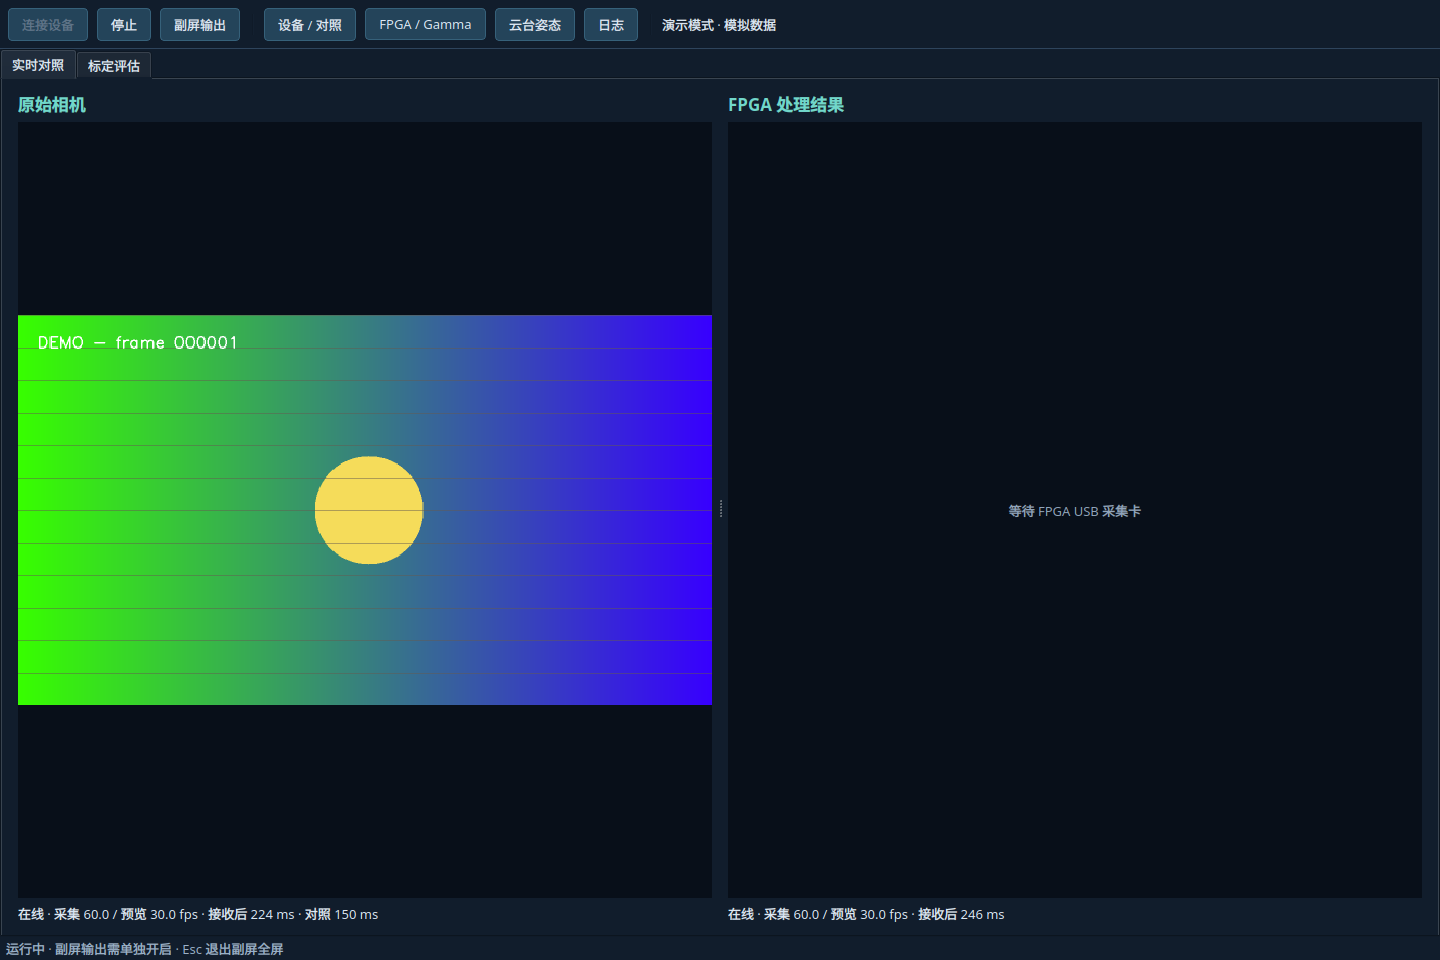
\includegraphics[width=\textwidth]{appendix/appendixC/figures/host_demo.png}
\caption{上位机主页布局（引用工程演示模式截图，画面和状态均不作为硬件测量数据）}
\label{fig:app-host-demo}
\end{figure}

\section{软件分层与并发设计}
\subsection{模块划分}
\begin{table}[htbp]\centering\small
\caption{上位机代码结构与职责}\label{tab:app-host-architecture}
\begin{tabularx}{\textwidth}{>{\raggedright\arraybackslash}p{3.0cm}Y}
\toprule
目录或模块 & 实现职责 \\
\midrule
\path{app.py}、\path{config.py} & 启动参数、设备发现、配置校验及 JSON 原子保存 \\
\path{core/protocols.py} & FPGA 包与 IMU 字节流的编解码、状态和统计数据类型 \\
\path{core/requests.py} & 单个未完成请求门控、序号匹配与超时 \\
\path{core/buffering.py}、\path{jpeg.py} & 带本地时间的有界历史、JPEG 增量分帧 \\
\path{core/model.py} & URDF/STL 资源解析、关节变换和显示网格简化 \\
\path{devices/} & 视频/串口后台 I/O、设备生命周期、演示数据及评估调度 \\
\path{evaluation/} & 标定文件转换、棋盘格检测、几何误差与相对 SFR；不依赖 Qt \\
\path{ui/} & 双图显示、独立工具窗口、评估结果和用户操作 \\
\bottomrule
\end{tabularx}
\end{table}

协议层与 I/O、界面分离，便于在没有 FPGA 或相机时测试解析器。
工作线程通过带锁快照发布状态，Qt 对象只在主线程更新。
视频采用最新帧邮箱和有界历史，界面定时拉取，
不为每个采集帧排队发送大量绘制事件，以防界面阻塞后积累过期图像。

\subsection{采集、预览和副屏分别调度}
每个视频源将连续读取、预览解码和全尺寸输出解码分开。
Linux 自动后端优先使用 FFmpeg/V4L2；MJPG 模式直接保留设备输出的 JPEG，
读取线程不做全尺寸解码或重新编码。
JPEG 分帧器支持分块输入、转义、重启标记和渐进多扫描，限制单帧大小，
不能简单搜索所有字节中的 \texttt{FFD8/FFD9} 代替完整分帧。
其他支持格式包括 YUYV、NV12，并提供 OpenCV 后端。

主页预览后台最多约 30 Hz，MJPG 先半尺寸解码再缩至 $640\times360$；
处理跟不上时跳过旧帧，保持最新画面。
副屏可见时独立解码最新全尺寸原始帧，使用 16 ms 定时器请求绘制，
不读取主页的对照延时。
采集卡只用于处理结果预览，不反向成为 FPGA 输入源。

原始相机历史最多保留 2.5 s 且不超过 128 MiB，
采集卡历史最多 0.25 s 且不超过 128 MiB；实际时间范围可能因码率提前缩短。
MJPG 历史保存压缩帧，其他格式保留缩小预览历史。
断连增加会话标识，后台结果只有在会话和设置仍匹配时才发布，
防止旧解码任务在清空后重新填入过期帧。

\subsection{延时对照与性能数据含义}
对照延时范围为 0--2000 ms，默认 150 ms，
只延迟原图预览，以便人工对齐 FPGA/采集卡链路的较晚画面。
选帧依据 PC 本地单调时钟，不具备硬件帧配对能力。
实时性检查时应将该值设为 0 ms，并分别观察实际采集率、预览发布率和帧龄。

界面的“接收后”时间从 PC 收到输入帧开始计，
包含配置延时、解码和界面调度，不包含设备内部或 USB 上游时间，
不能作为 FPGA 端到端延迟。
同样，请求 1080p60、每 16 ms 请求绘制和实际 HDMI 输出频率是不同事件；
副屏物理时序应在操作系统显示设置中确认，应用不会自动修改显示模式。
\sourcefile{\path{../PC/fpga_host/devices/video.py}；
\path{../PC/fpga_host/devices/video_sources.py}；
\path{../PC/fpga_host/core/buffering.py}；
\path{../PC/docs/development.md}}

\section{FPGA 控制与 Gamma 遥测}
\subsection{协议与帧边界生效}
FPGA 控制包使用二进制格式
\begin{center}\small
\texttt{A5 5A | VERSION | TYPE | SEQ | LEN | PAYLOAD | XOR}。
\end{center}
VERSION 为 \texttt{01}，XOR 从 VERSION 到载荷末尾逐字节异或，
多字节统计字段为小端。
\texttt{SET\_FEATURES/GET\_STATUS/SET\_STREAM/GET\_SNAPSHOT}
分别为 \texttt{10/11/12/13}，返回
\texttt{STATUS/GAMMA\_STATS} 为 \texttt{80/81}，以上编号均为十六进制。
STATUS 负载为 8 字节，Gamma 统计负载为 28 字节。

功能掩码 bit0、bit1、bit2 分别控制去畸变、姿态矫正和自动 Gamma，
上位机一次提交完整三位掩码，禁用设备 \path{available_mask} 不支持的位。
界面同时显示 requested、applied 和 pending：请求已接收后，
还要等输入 SOF 才应用于后续完整输入帧。
applied 变化也不意味着该帧的矫正结果已经出现在 HDMI 上。

\path{RequestGate} 只允许一个未完成请求，
只有序号匹配且负载合法的 STATUS 才释放门控；
异步 Gamma 统计或旧序号响应不能冒充 ACK。
连接后及每 250 ms 查询状态，用户命令优先于下一次轮询，
pending 期间禁止重复提交 SET，仍允许查询和遥测操作。
1 s 内未收到匹配响应时断开，约 2 s 后重连并查询实际状态，
不自动重放 SET，以应对命令已执行但 ACK 丢失的情况。

\subsection{亮度统计与新鲜度}
遥测包括输入帧编号、有效像素数、增强前后亮度和、
增强前暗部/高光计数、实际/目标曲线与该帧功能掩码。
平均亮度与比例分别由亮度和、计数除以有效像素数得到，
分母为零时显示无效，不能显示为零亮度。
暗部和高光比例都来自增强前图像，不能直接解释为增强后比例改善。

Gamma 曲线视图按协议公式绘制示意，
不是从 FPGA LUT 逐项读取的结果；关闭增强时显示恒等映射。
软件分别记录最近合法统计包接收时间和最近帧编号变化时间，
避免重复发送旧统计时误报“图像持续更新”。
这些统计属于输入 Gamma 阶段，不能与最终 HDMI 显示帧默认建立一一对应。
\sourcefile{\path{../PC/fpga_host/core/protocols.py}；
\path{../PC/fpga_host/core/requests.py}；
\path{../PC/fpga_host/devices/serial_link.py}；
\path{../PC/Device/fpga_uart/reference/pc_control_protocol.md}}

\section{姿态解码与三维模型显示}
STM32 接收端按附录~\ref{app:attitude-estimation}~的十字节协议增量解码，
支持半帧、多帧、噪声与错误校验后的重新同步。
三轴补码除以 2048 得到弧度，再转换成界面角度；
连续 0.5 s 无合法帧时标记超时，数值置为无效，模型保留最后姿态。
由于协议没有采样时间戳和就绪位，即使通信持续，也不能确认传感器数据持续更新。

模型视图读取已有 URDF 与 STL，按 joint origin、axis 和关节层级组合刚体变换，
支持资源中的 \texttt{package://} 路径，不依赖 ROS 或 OpenGL。
当前 yaw/pitch 关节随姿态运动，原模型无 roll 关节，roll 仅以读数显示。
视图采用 CPU QPainter 正交投影、深度排序和简化网格，用于观察方向和零位。

用户可设置 yaw/pitch 显示方向，并将当前姿态设为模型零点。
该操作只影响本次连接中的 PC 显示，不会改变原始读数、固件校准或 FPGA 矫正参数，
断开后零点清除。
模型显示也不包含已标定的相机--IMU 外参，
必须按实际安装完成轴向检查后，才可辅助判断相机姿态。
\sourcefile{\path{../PC/fpga_host/core/model.py}；
\path{../PC/fpga_host/ui/widgets.py}；
\path{../PC/Device/imu_usbdcdc/reference/usb_receive_manual.md}}

\section{图卡评估模块与标定结果导入}
\subsection{全分辨率检测和指标计算}
评估页支持原始相机、FPGA 采集卡和静态图像，默认图卡为 $9\times6$ 个内角点。
实时模式约每秒选取一张不同序号的最新帧，连续三次检测稳定，
相邻检测的角点运动 RMS 小于 1.5 px 后自动评估。
检测丢失或输入超时会清除旧报告，避免将上一次有效值留作当前结果。
静态图与演示图直接评估一次，不做运动稳定性判断。

检测可以先缩小图像搜索角点，但会在原尺寸上细化，
直线度与 SFR 均使用原始分辨率，不能从主页 $640\times360$ 缩略图计算。
几何模块沿棋盘格实际灰度边缘搜索梯度峰并亚像素定位，
对整行和整列做正交直线拟合，统计 RMS、P95 和最大距离；
另提供角点直线度、网格单应拟合及导入内参后的重投影残差。

SFR 模块选择最多 24 条分散斜边，提取 ESF/LSF，经窗函数、FFT 和导数响应补偿，
报告各边 SFR、MTF50 与过冲/欠冲。
允许的斜边倾角为 $1.5^\circ$--$15^\circ$，建议约 $5^\circ$；
对低对比度、饱和、ROI 太小、亚像素覆盖不足或无有效交点等情况记录无效原因。
亮度响应未知时输出编码亮度下的相对 SFR，
仅在明确相机响应时选择线性或 sRGB 近似反响应。

\begin{figure}[htbp]\centering
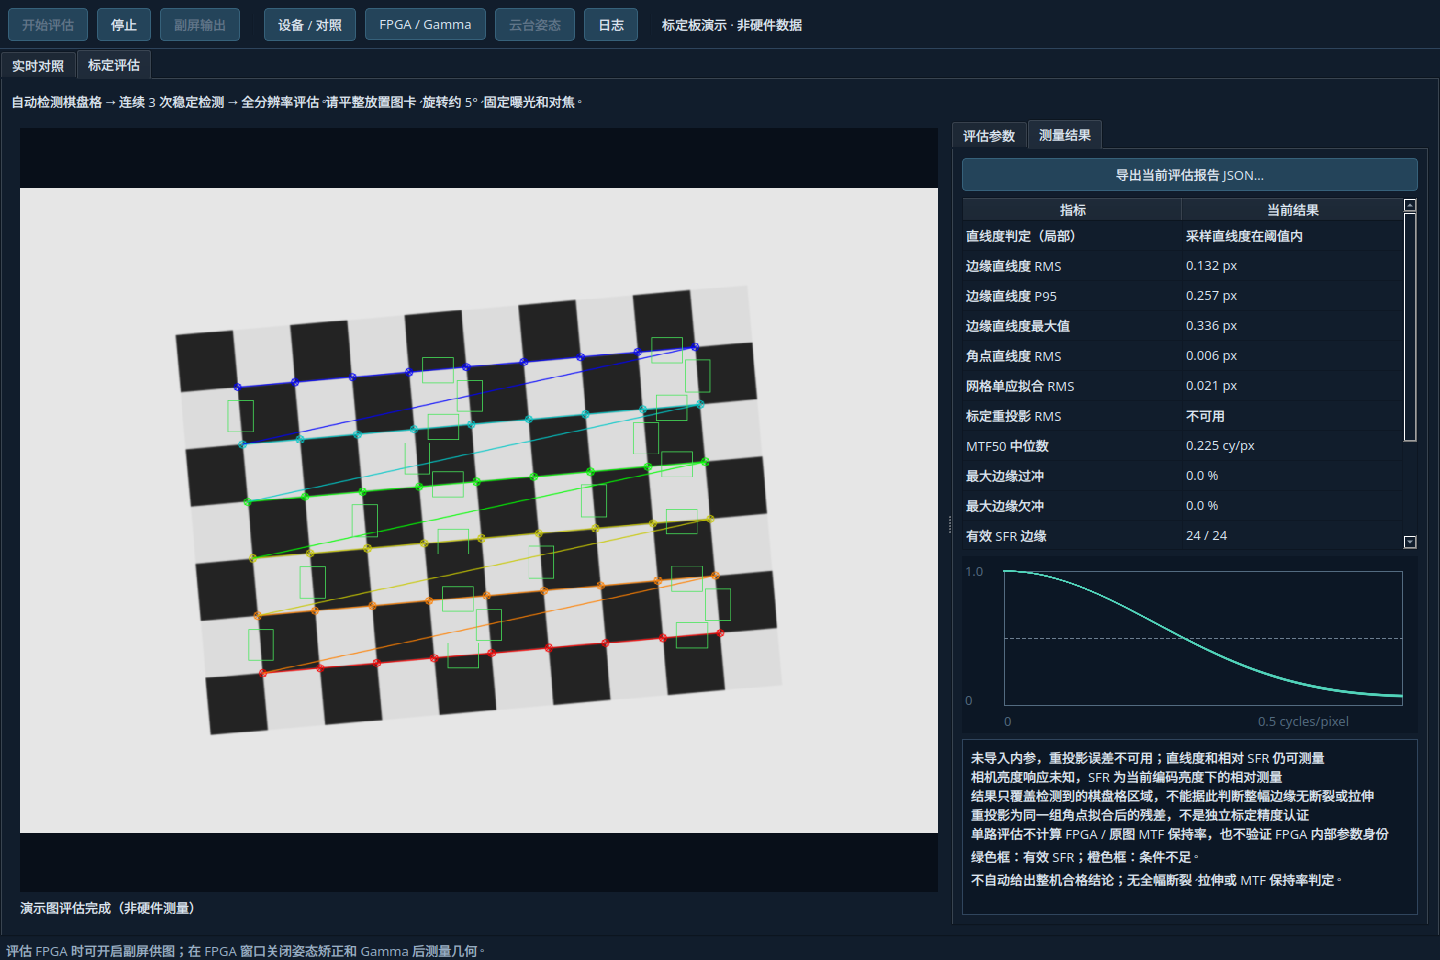
\includegraphics[width=\textwidth]{appendix/appendixC/figures/host_evaluation_demo.png}
\caption{图卡评估界面（工程合成棋盘格演示；图内数值不作为相机或 FPGA 实测结果）}
\label{fig:app-host-evaluation}
\end{figure}

局部直线度默认参考阈值为 RMS 不超过 0.30 px、P95 不超过 0.50 px，
有效边缘采样率至少 80\% 才给出局部阈值判断。
这些值是软件可调整的初始设置，正式验收应采用第~\ref{chap:performance}~章
事先确定的门限，不将默认值写成赛题官方标准。
当前实现不是经过认证的 ISO 12233 测量工具，
也不自动评估整幅拉伸、断裂或给出整机合格结论。

\subsection{标定参数与 JSON 报告}
标定解析器支持附录~\ref{app:camera-calibration}~的 MATLAB JSON，
也支持 OpenCV Brown 模型的 JSON 和 YAML 文件。
MATLAB 内参先转置，再按显式像素起点将主点减 1；
不支持的鱼眼、非零 skew 等模型应拒绝，
图像尺寸不符时不自动缩放内参。
已矫正图像使用实际输出内参和零畸变系数进行参考重投影，
原始图像才允许额外的软件去畸变，避免重复处理。

导入参数只用于 PC 分析，不下发 FPGA，也不能证明硬件内部参数一致。
输出 JSON 保留图像尺寸、图卡、输入几何、软件参考开关、
参数路径与 SHA256、实际 K/D、逐边 ROI 与 SFR、无效原因、阈值和输入接收信息。
对采集卡可附带分析前查询到的功能状态，
但串口状态与视频没有硬件逐帧同步，当前也不计算同步原图/FPGA 图的 MTF 保持率。

导出操作应在停止或切换页面之前进行；
目前 JSON 不包含原始图像，需另外保存原图、曝光/格式、图卡位置和 FPGA 位流信息，
才能按第七章方案复核测量条件。
\sourcefile{\path{../PC/fpga_host/evaluation/}；
\path{../PC/fpga_host/devices/evaluation.py}；
\path{../PC/docs/evaluation.md}}

\section{部署、联调与软件验证}
\subsection{启动与实物操作流程}
在 PC 工程目录建立 Python 虚拟环境并安装 \path{requirements.txt}，
依赖为 PySide6-Essentials、NumPy、opencv-python-headless 和 pyserial。
Linux 硬件模式建议准备 FFmpeg、v4l2-ctl 和 xrandr，
采用 headless OpenCV 可避免其 Qt 插件与 PySide6 冲突。
常用启动命令为
\begin{quote}\small\ttfamily
python -m fpga\_host --demo\\
python -m fpga\_host --config ./settings.json
\end{quote}
首条命令用于无设备界面演示，第二条使用指定配置运行硬件模式。
配置按版本和字段类型校验，并以临时文件替换方式保存；
设备或模型设置应在停止后修改。

\begin{enumerate}
\item 核对 USB 相机、HDMI 采集卡、CP210x 与 STM32 CDC 为正确且不同的设备节点，
下载支持当前协议的 FPGA 位流并启动 STM32 固件。
\item 在系统中启用独立扩展副屏，确认物理信号为 $1920\times1080$、约 60 Hz，
再选定副屏名称；避免镜像、桌面缩放或远程桌面改变输出条件。
\item 连接设备，分别检查两路实际采集与预览 fps，打开副屏输出向 FPGA 供图。
\item 查询 FPGA 状态，提交功能掩码，等待 pending 清除，
再观察输出变化；无输入 SOF 时保留等待提示。
\item 转动 IMU 检查三轴正负号，用模型方向和零点设置辅助观察，
同时按附录~\ref{app:attitude-estimation}~核对实际相机坐标。
\item 定量评估时固定图卡、对焦、曝光与格式，关闭姿态矫正及 Gamma，
采用明确的去畸变开关和输入几何设置，保存全分辨率图像与 JSON。
\end{enumerate}

\subsection{本次软件测试结果}
2026 年 10 月 25 日，使用 PC 工程已有虚拟环境，在 Qt offscreen 模式执行
\begin{quote}\small\ttfamily
QT\_QPA\_PLATFORM=offscreen \textbackslash{}\\
python -B -m unittest discover -s tests -v
\end{quote}
该命令在 PC 工程根目录运行，反斜杠表示 shell 续行。
本次 51 项测试全部通过，无失败或跳过，耗时约 41.3 s。
测试日志与源码身份记录保存在 \path{appendix/references/}。

\begin{table}[htbp]\centering\small
\caption{本次上位机自动测试结果}\label{tab:app-host-tests}
\begin{tabularx}{\textwidth}{>{\raggedright\arraybackslash}p{3.0cm}cY}
\toprule
测试文件 & 数量 & 主要检查内容（均通过） \\
\midrule
\path{test_protocols.py} & 12 & 协议样例、拆包/粘包、噪声重同步、有符号角度、统计合法性及序号门控 \\
\path{test_core.py} & 7 & 缓冲时间/容量、配置校验、实际 URDF 资源和关节变换、显示模式识别 \\
\path{test_serial.py} & 2 & POSIX 虚拟串口、遥测与 ACK 交错、pending、无响应超时及不重放 SET \\
\path{test_video.py} & 10 & JPEG 分帧、FFmpeg 管道、慢解码跳帧、预览延时与副屏独立、断连失效 \\
\path{test_evaluation.py} & 12 & MATLAB/OpenCV 参数、解析高斯斜边、弯曲网格、重投影及评估取消 \\
\path{test_ui.py} & 8 & Qt 演示交互、双路后台解码、页面互斥、静态输入及 JSON 导出 \\
\bottomrule
\end{tabularx}
\end{table}

以上测试验证软件解析、数值趋势、线程调度及界面行为。
合成高斯斜边和棋盘格通过，不代表真实图卡的 MTF50 或直线度已经达标；
虚拟串口通过，也不能替代实际 USB、双屏物理时序与设备断连测试。
实物联调仍需记录两路采集格式和吞吐、正确的副屏输出、长时间运行、
拔插恢复、实际图卡评估与最终 FPGA 位流身份。
\sourcefile{\path{../PC/tests/}；
\path{appendix/references/pc_unittest_20261025.txt}；
\path{appendix/references/source_manifest_20261025.json}}
